\documentclass[12pt,a4paper]{article}
\usepackage[polish]{babel}
\usepackage[T1]{fontenc}
\usepackage[utf8x]{inputenc}
\usepackage{hyperref}
\usepackage{url}
\usepackage[]{algorithm2e}
\usepackage{listings}
\usepackage{graphicx}
\usepackage{color}
\usepackage{listings}
\usepackage{multirow}
\usepackage{hyperref}

\lstloadlanguages{% Check Dokumentation for further languages ...
	C,
	C++,
	csh,
	Java
}

\definecolor{red}{rgb}{0.6,0,0} % for strings
\definecolor{blue}{rgb}{0,0,0.6}
\definecolor{green}{rgb}{0,0.8,0}
\definecolor{cyan}{rgb}{0.0,0.6,0.6}

\lstset{
	language=csh,
	basicstyle=\footnotesize\ttfamily,
	numbers=left,
	numberstyle=\tiny,
	numbersep=5pt,
	tabsize=2,
	extendedchars=true,
	breaklines=true,
	frame=b,
	stringstyle=\color{blue}\ttfamily,
	showspaces=false,
	showtabs=false,
	xleftmargin=17pt,
	framexleftmargin=17pt,
	framexrightmargin=5pt,
	framexbottommargin=4pt,
	commentstyle=\color{green},
	morecomment=[l]{//}, %use comment-line-style!
	morecomment=[s]{/*}{*/}, %for multiline comments
	showstringspaces=false,
	morekeywords={ abstract, event, new, struct,
		as, explicit, null, switch,
		base, extern, object, this,
		bool, false, operator, throw,
		break, finally, out, true,
		byte, fixed, override, try,
		case, float, params, typeof,
		catch, for, private, uint,
		char, foreach, protected, ulong,
		checked, goto, public, unchecked,
		class, if, readonly, unsafe,
		const, implicit, ref, ushort,
		continue, in, return, using,
		decimal, int, sbyte, virtual,
		default, interface, sealed, volatile,
		delegate, internal, short, void,
		do, is, sizeof, while,
		double, lock, stackalloc,
		else, long, static,
		enum, namespace, string},
	keywordstyle=\color{cyan},
	identifierstyle=\color{red},
}
\usepackage{caption}
\DeclareCaptionFont{white}{\color{white}}
\DeclareCaptionFormat{listing}{\colorbox{blue}{\parbox{\textwidth}{\hspace{15pt}#1#2#3}}}
\captionsetup[lstlisting]{format=listing,labelfont=white,textfont=white, singlelinecheck=false, margin=0pt, font={bf,footnotesize}}


\addtolength{\hoffset}{-1.5cm}
\addtolength{\marginparwidth}{-1.5cm}
\addtolength{\textwidth}{3cm}
\addtolength{\voffset}{-1cm}
\addtolength{\textheight}{2.5cm}
\setlength{\topmargin}{0cm}
\setlength{\headheight}{0cm}

\begin{document}
	
	\title{Programowanie obiektowe i graficzne\\\small{dokumentacja projektu NutritionApp}}
	\author{Dariusz Momot \\ Łukasz Kudzia \\ grupa 2E}
	\date{\today}

	\maketitle
	\newpage
	\section*{Część I}
	\subsection*{Opis programu}
	NurtritionApp to narzędzie pomagające w planowaniu posiłków oraz listy zakupów na dany tydzień.
	Program posiada podstawową listę przepisów, którą można modyfikować poprzez dodawanie lub usuwanie wybranego przepisu.
	Podczas planowania posiłków na dany tydzień można skorzystać z już stworzonych przepisów.
	Przy tak stworzonym planie w zakładce \textit{Grocery List} możemy zobaczyć listę zakupów potrzebnych na wybrane posiłki,
	w której możemy usunąć produkty już posiadane w lodówcę a następnie zapisać listę zakupów w pliku o rozszerzeniu \textit{pdf}.
	
	\subsection*{Instrukcja obsługi}
	Aby uruchomić program należy podwójnie kliknąć w plik o nazwie \textbf{NutritionApp.exe} znajdujący się w folderze 
	z programem. \\Po uruchomieniu programu ukażę się menu po lewej stronie wraz z dostępnymi zakładkami. \\
	W zakładce Planner możemy ustalić posiłki na poszczególne dni, wybierając dzień po lewej stronie a następnie klikając w 
	w przyciski odpowiedzialny za poszczególne posiłki. W razie gdy chcemy usunąć konkretny przepis wystarczy zaznaczyć go, a 
	nastepnie kliknąć \textit{Delete Recepies}. \\
	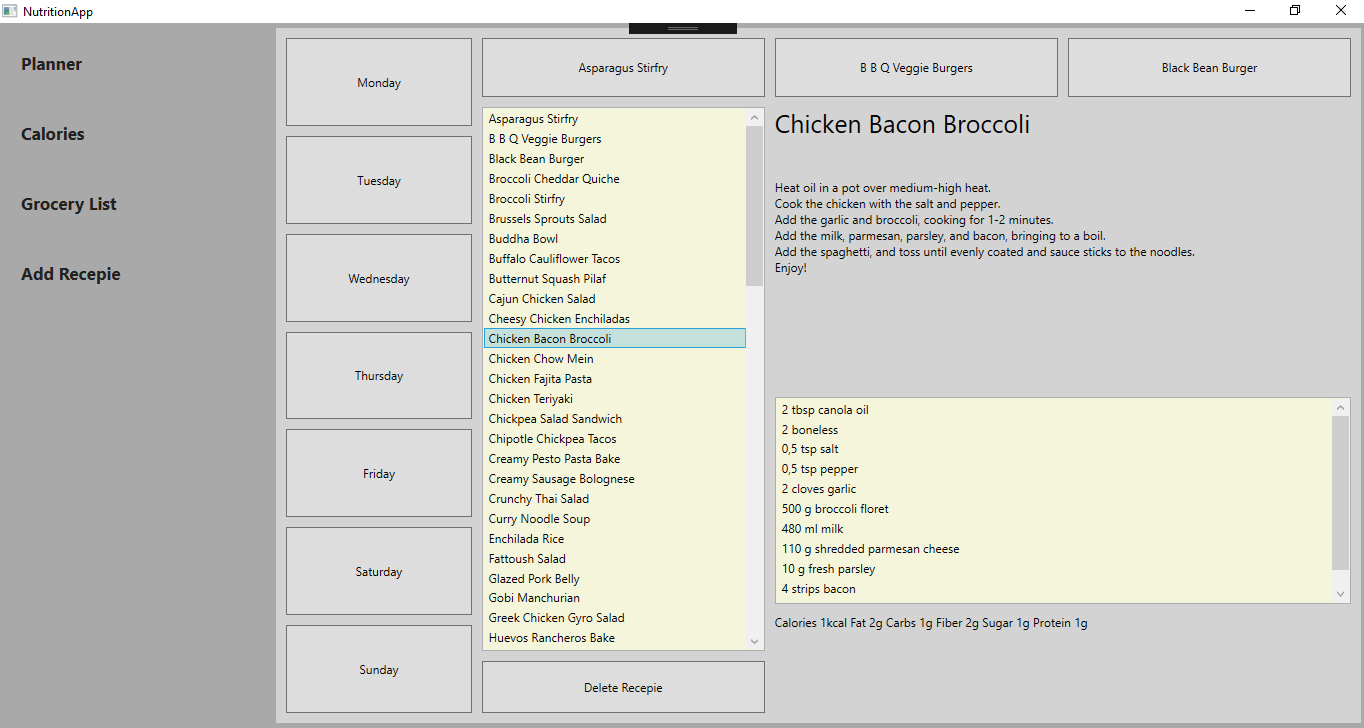
\includegraphics[scale = 0.5]{img/Planner.png} 
	\newpage
	
	W zakładcę \textit{Calories} możemy zobaczyć ilość słakładników odżywczych na poszczegolne dni oraz całkowite podsumowanie
	w tygodniu.\\
	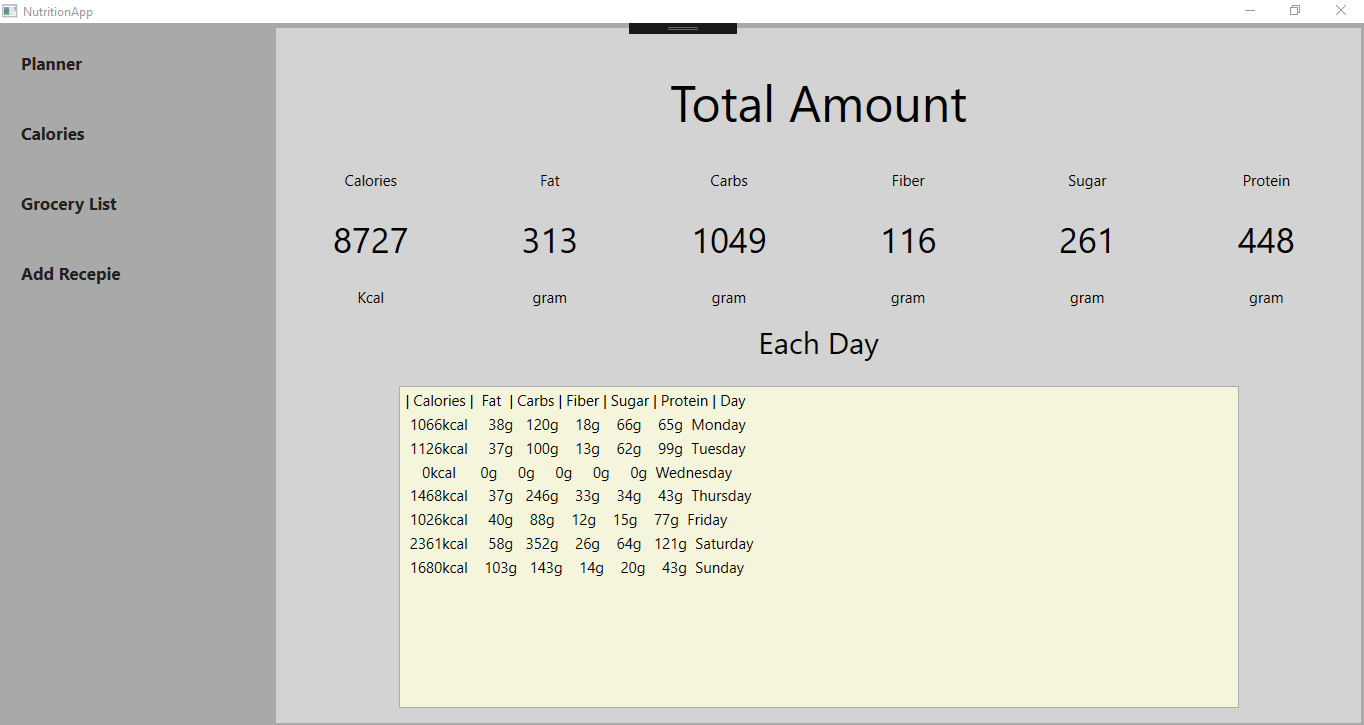
\includegraphics[scale = 0.5]{img/Calories.png} \\
	
	Zakładka \textit{Grocery list} oferuję podgląd listy zakupów wymaganych w przepisach, w której poszczególne składniki 
	możemy usunąć zaznaczając go na liście a następnie klikając w przycisk o nazwię \textbf{Delete}.
	Aby stworzyć listę zakupów klikamy w przycisk \textbf{Print}, następnie wybieramy docelowe miejsce zapisu pliku w formacie 
	\textit{.pdf}. \\
	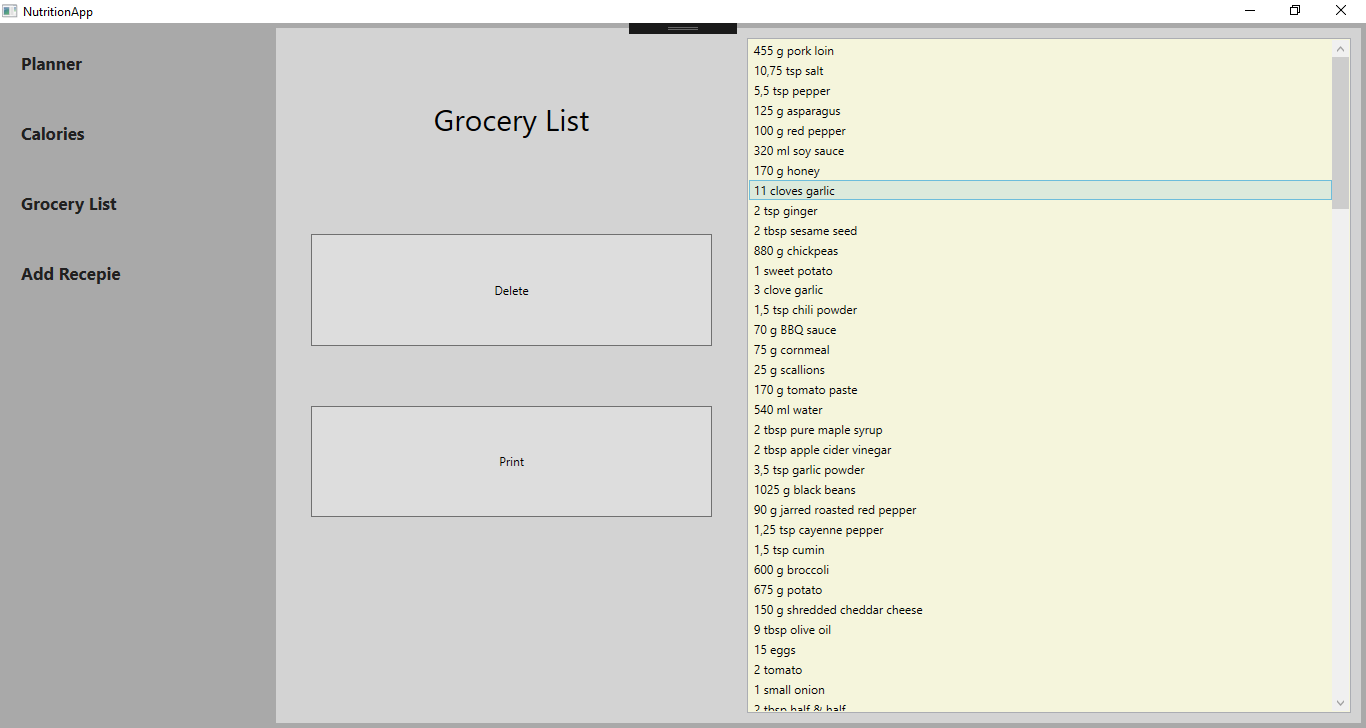
\includegraphics[scale = 0.5]{img/GroceryList}\\ 

	W zakładcę \textit{Add Recepie} możemy dodać przepis, wystarczy że uzupełnić nazwę przepisu, instrukcję wykonania, 
	dodać składniki wymagane w przepisie oraz dodać skłądniki odżywcze danego przepisu. W razie pomyłki przy dodawaniu 
	składnika możemy go usunąć w przycisku nad listą składników \\
	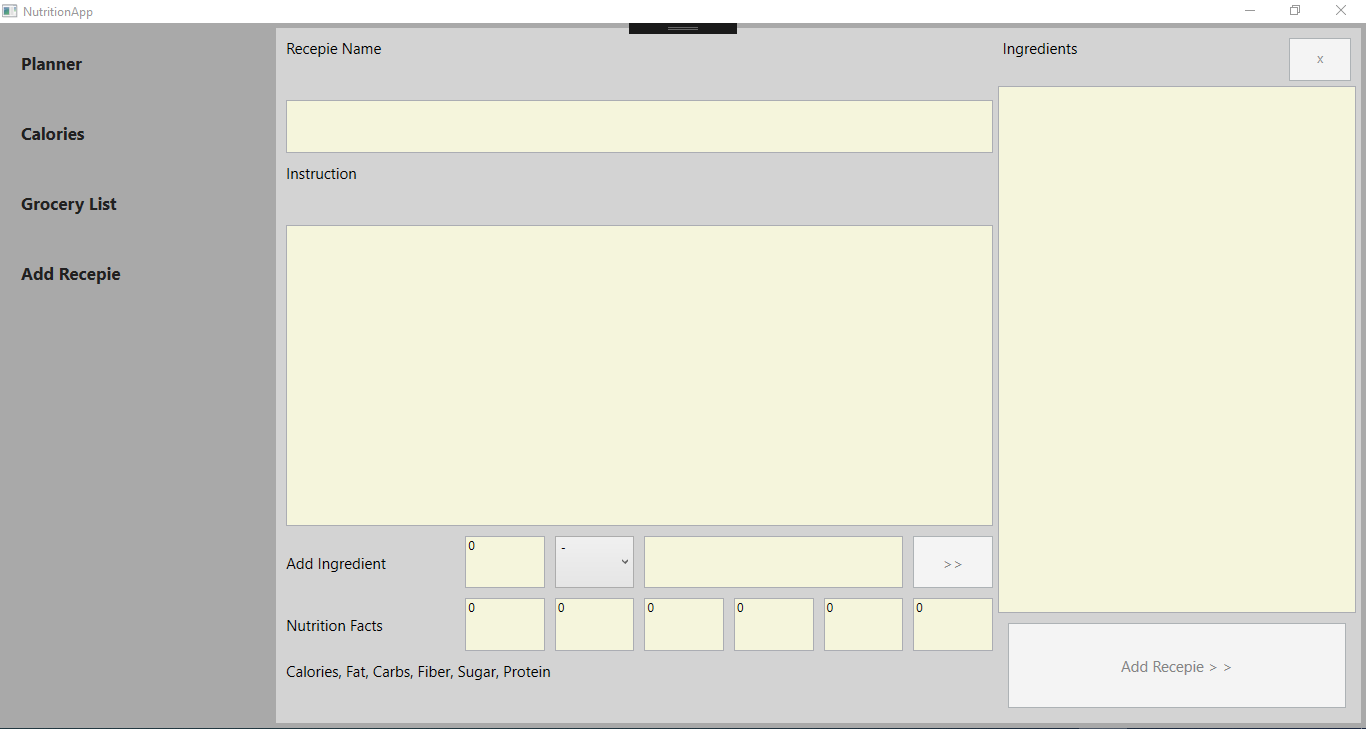
\includegraphics[scale = 0.5]{img/AddRecepie.png} \\
	\newpage

	\section*{Część II}
	\subsection*{Lista zadań} 
	\begin{table}[h]
\caption{Wykaz zadań i prac zrealizowanych w zespole}
\label{tab:my-table}
\begin{tabular}{|c|c|c|}
\hline
Imię Nazwisko                   & Odpowiedzialny za                                                                                                & Zrealizował zadania                                                                                \\ \hline
\multirow{9}{*}{Łukasz Kudzia}  & \multirow{3}{*}{\begin{tabular}[c]{@{}c@{}}1. Możliwość wybierania posiłków na \\ poszczególne dni\end{tabular}} & \begin{tabular}[c]{@{}c@{}}1. Dodanie funkcjonalności \\ wybierania przepisów\end{tabular}         \\ \cline{3-3} 
                                &                                                                                                                  & 2. Zbindował widok z VM                                                                            \\ \cline{3-3} 
                                &                                                                                                                  & 3. Stworzenie podstawowych klas                                                                    \\ \cline{2-3} 
                                & \multirow{3}{*}{2. Stworzenie widoku aplikacji}                                                                  & 1. Dodanie widoku Planner                                                                          \\ \cline{3-3} 
                                &                                                                                                                  & 2. Dodanie widoku Calories                                                                         \\ \cline{3-3} 
                                &                                                                                                                  & 3.Dodanie widoku Add Recepies                                                                      \\ \cline{2-3} 
                                & \multirow{3}{*}{3. Testowanie}                                                                                   & \begin{tabular}[c]{@{}c@{}}1. Testowanie funkcjonalności dodawania\\ przepisów\end{tabular}        \\ \cline{3-3} 
                                &                                                                                                                  & \begin{tabular}[c]{@{}c@{}}2. Testowanie funkcjonalności drukowania\\ listy zakupów\end{tabular}   \\ \cline{3-3} 
                                &                                                                                                                  & \begin{tabular}[c]{@{}c@{}}3. Testowanie funkcjonalności zapisu ,\\ odczytu przepisów\end{tabular} \\ \hline
\multirow{10}{*}{Dariusz Momot} & \multirow{2}{*}{1. Funkcjonalność zapisu odczytu}                                                                & 1. Dodanie odczytu  i zapisu                                                                       \\ \cline{3-3} 
                                &                                                                                                                  & 2. Bindowanie listu przepisu do widoku                                                             \\ \cline{2-3} 
                                & \multirow{3}{*}{\begin{tabular}[c]{@{}c@{}}2. Funkcjonalność podglądu \\ wartości odżywczych\end{tabular}}       & 1. Dodanie widoku Calories                                                                         \\ \cline{3-3} 
                                &                                                                                                                  & 2. Sumowanie wartości odżywczych                                                                   \\ \cline{3-3} 
                                &                                                                                                                  & 3. Bindowanie widoku                                                                               \\ \cline{2-3} 
                                & \multirow{2}{*}{\begin{tabular}[c]{@{}c@{}}3. Funkcjonalność drukowania \\ listy przepisów\end{tabular}}         & \begin{tabular}[c]{@{}c@{}}1. Zapoznanie się z biblioteką\\ ITextShapr\end{tabular}                \\ \cline{3-3} 
                                &                                                                                                                  & 2. Dodanie drukowania przepisów                                                                    \\ \cline{2-3} 
                                & \multirow{2}{*}{4. Testowanie}                                                                                   & \begin{tabular}[c]{@{}c@{}}1. Testowanie poprawnego bindowania \\ widoków\end{tabular}             \\ \cline{3-3} 
                                &                                                                                                                  & 2. Testowanie planowania przepisów                                                                 \\ \cline{2-3} 
                                & 5. Inne                                                                                                          & 1. Dodanie modelu Singleton                                                                        \\ \hline
\end{tabular}
\end{table}
	
	\subsection*{Przebieg rezalizacji}
	W trakcie planowania projektu, z góry założyliśmy że program jaki napiszemy zostanie napisany w oparciu o architekturę MVVM.
	Do zapisu oraz odczytu listy przepisów użyliśmy \textbf{Newtonsoft.JSON}, a do drukowania listy zakupów w postaci .pdf
	posiłkowaliśmy się biblioteką \textbf{ITextSharp}. Proces komunikacji przebieg bez problemów a z racji na niewielką liczność grupy
	używaliśmy komunikatora \textit{Messenger}. Do pracy przy projekcie używalismy najpopularnieszego systemu kontroli 
	wersji jakim jest \textit{git}. Podczas pracy nad projektem skorzystaliśmy ze wzorca \textbf{Singleton}, który ułatwił nam 
	prace związaną z listą przepisów. Podczas pracy gdy jedna osoba napisała jakąś funkcjonalność, druga testowała pod kątem 
	ewentualnych błędów.\\ \\

	\textbf{Łukasz Kudzia} odpowiedzialny głównie za stworzenie widoków oraz ich bindowanie. Stworzył również logikę 				odpowiedzialną za planowanie posiłków. Pomysłodawca projektu oraz lider zespołu. \\ \\

	\textbf{Dariusz Momot} odpowiedzialny za logikę podliczania kalorii, wczytywanie oraz zapis do pliku listy przepisów.
	Zaimplementował zworzec singleton wraz z zapisaniem listy zakupów do pliku pdf. 

	
	\subsection*{Podsumowanie i wnioski}
	Projekt został zrealizowany w podstawowym jego założeniu, jakim było dodawanie, usuwanie przepisów, wyszczególnienie wartości odżywczych na poszczególne dni wraz z drukowaniem listy zakupów. Najwięcej problemów sprawiało bindowanie elementów, wynikało z niepoprawnie pisanego kodu na początku, przez co każda zmiana zajmowała więcej czasu niż powinna. Kolejnym problemem był transport danych pomiędzy widokami. \\
Jako dalszy rozwój zaplanowaliśmy stworzenie bazy danych zawierającej użytkowników wraz z ich listą przepisów oraz bazy danych ze 
składnikami wraz z ich wartościamy odżywczymi tak aby użytkownik nie musiał podawać ich samodzielnie. \\
	
	
	\subsection*{Udokumentowanie wykorzystania systemu kontroli wersji}
	Link do zdalnego repozytorium na Github'ie \href{https://github.com/Qdzia/NutritionAPP}{NurtitionApp} \\
	
	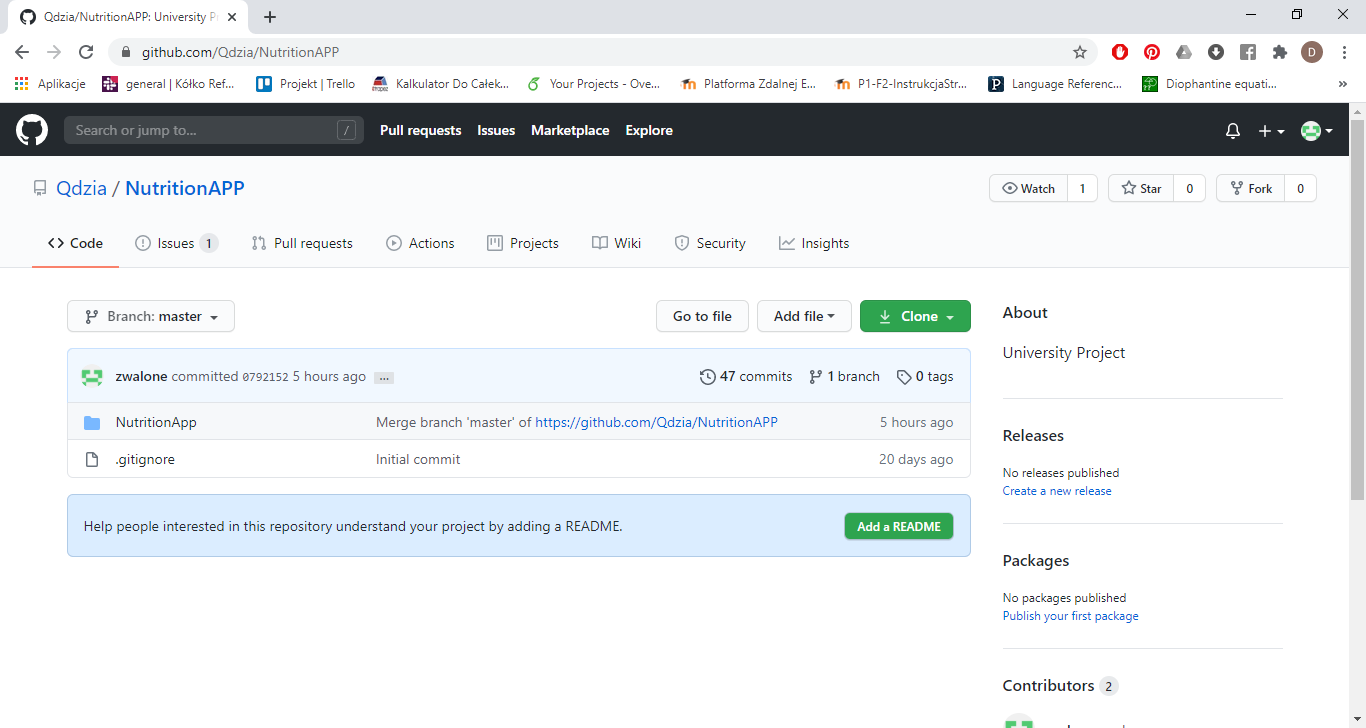
\includegraphics[scale = 0.5]{img/Git1.png}\\ 
	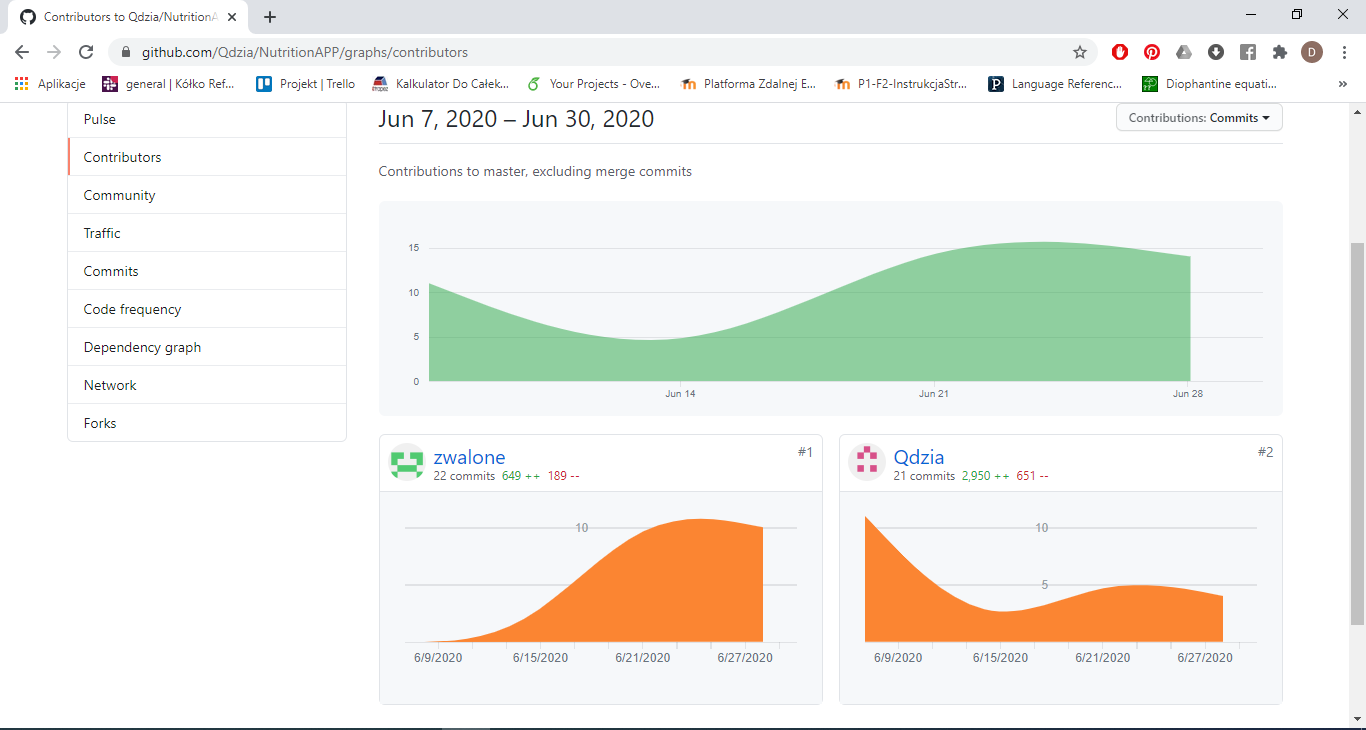
\includegraphics[scale = 0.5]{img/Git2.png} 
	

\end{document}
